\section{Design Brief and Method for the Dynamic Honeycomb Maze}

\subsection{Hexgonal Grid}
% Section about the grid upon which the robots are placed

As shown in Figure \ref{fig:hexgrid_with_numbers}, on the floor of the experimentation room where the robots are placed, there is a hexagonal grid. There are notably light grey lines on a dark black background. The \textit{Khepera IV} robots (as see in Figure \ref{fig:robot}), is able to detect, and count, how many of the lines it has crossed duration rotation and during  

\begin{figure}
    \centering
    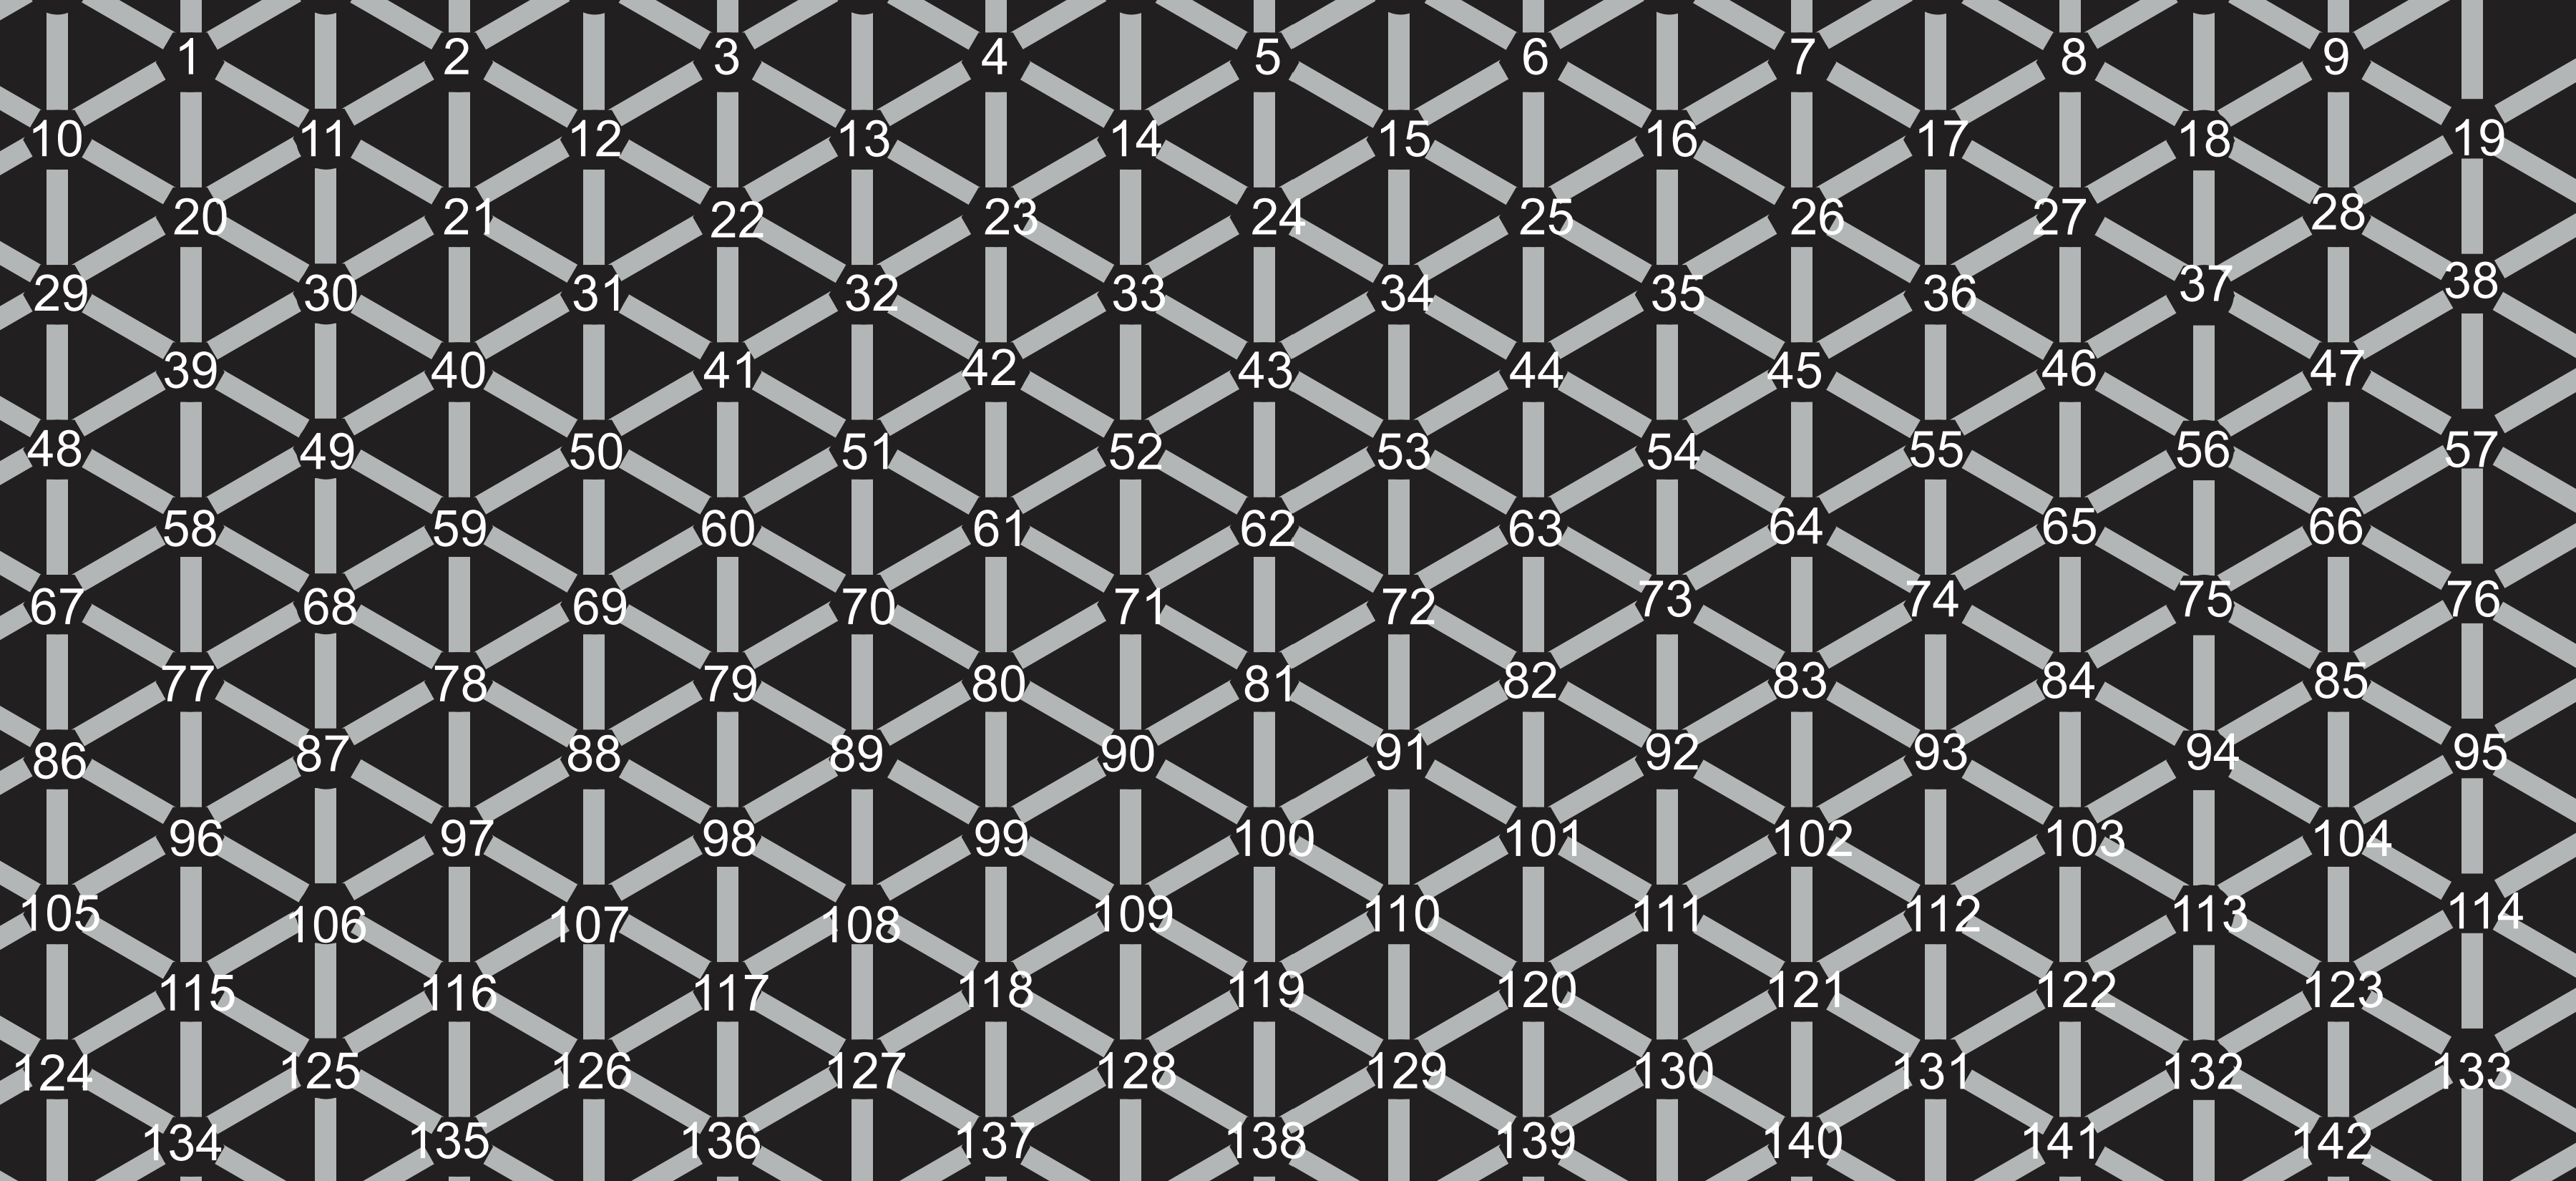
\includegraphics[scale = 0.3]{images/hexgrid_with_numbers.png}
    \caption{This shows the mat on the floor of the experimentation room which, upon which, the line following robots will navigate. The black and light grey lines can be detected by the line following robots' IR sensors.}
    \label{fig:hexgrid_with_numbers}
\end{figure}

\subsection{\textit{Khepera IV} Robots}


% Section about the Khepera IV robot, their design and hence the limitations
The robots used in this maze are the \textit{Khepera IV} robots. They are line following robots that have IR sensors on their bottom surface. THis allows robots to be able to detect when they have crossed a white line as shown in figure \ref{fig:hexgrid_with_numbers}

\begin{figure}
    \centering
    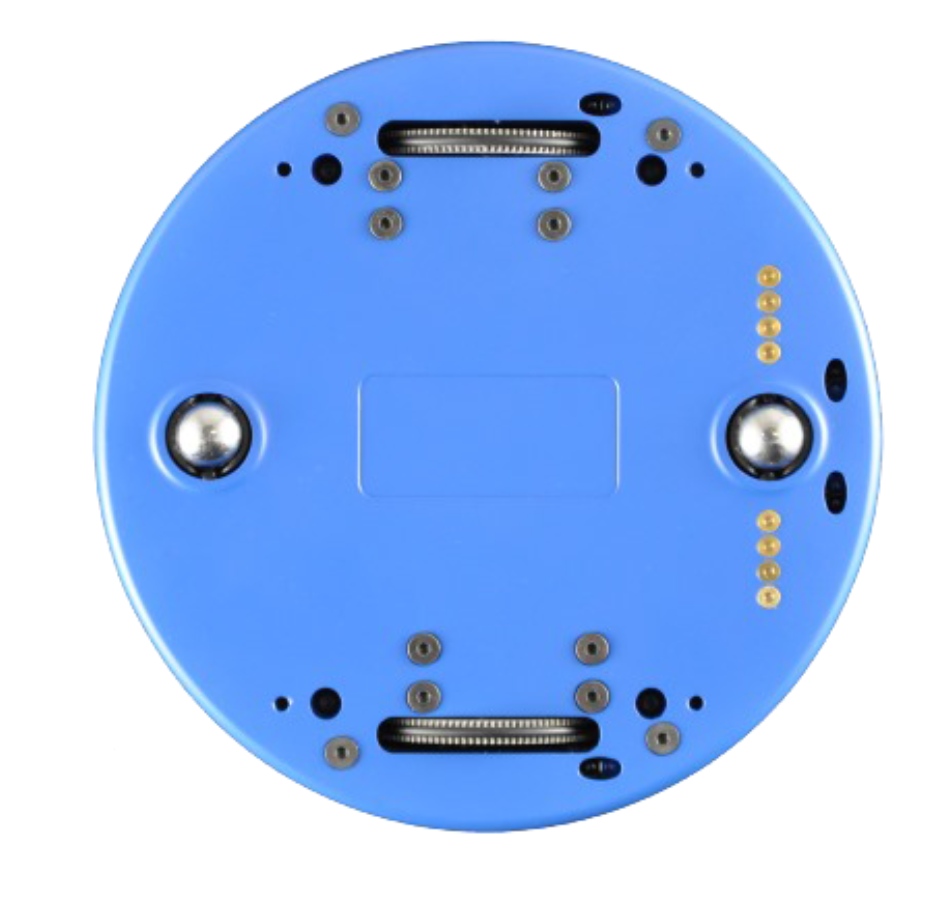
\includegraphics[scale = 0.5]{images/khepera_IV_robot.png}
    \caption{Shown is the underneath of the \textit{Khepera IV} robot. Note the presence of the 2 parralel wheels of the robot. This leads to signicant movement limitations of the \textit{Khepera IV} robots which must be addressed in the development of the program to control the Dynamic Honeycomb Maze.}
    \label{fig:robot}
\end{figure}

\subsection{Platforms}

%Section about the design of the platforms of the robot and the limitations that come with it
Intrinsic important design constraints to overcome in making the honeycomb maze:
\begin{enumerate}
    \item Due to the nature of the shape of the platforms, two hexagonal platform \textit{that are consecutive} are unable to rotate without colliding. To avoid this the hexagonal platform can not be consecutive to another platform robot when they rotate.
    \item Due to the design of the robot platform,  the robots have a sense of polarity. This is because they have a navigation style similar to tank treads where they can only move backwards and forwards, however can not simply move left and right without rotating first. 
\end{enumerate}


\subsection{Development Environment}

%Justify the use of python 


\subsection{Network of Integration}

% Explain how the python code will interact with the robots directly.

With input from \textit{deeplabcut}



As the aim of this dissertation is to develop a tool for investigating the behaviour of mouse models, is it also an important aim for the program to be structured such a way that modifications to the code to add new behaviour in the future are possible

Due to these design constraints, the problem becomes more challenging to solve. 

